\chapter{Conceptos Previos}

\section{Programaci\'on Orientada a Objetos}
La Programaci\'on Orientada a Objetos (POO) \cite{poo} es un paradigma de programaci\'on basado en el uso de clases\footnote{Plantillas para la creaci\'on de objetos que brinda los valores iniciales del estado (variables) y implementaciones de comportamiento (m\'etodos).} donde sus instancias son llamadas objetos. La idea principal en este paradigma es lograr crear, por medio del \textit{Software}, un sistema basado en componentes independientes que interact\'uen entre ellos de la misma forma que lo hace el sistema concreto a modelar. La programaci\'on orientada a objetos se basa en dise\~nar interacciones entre objetos para crear aplicaciones y sistemas inform\'aticos, usando diversas t\'ecnicas como la abstracci\'on, la herencia, el polimorfismo, la cohesi\'on, el acoplamiento y encapsulamiento. Un objeto busca modelar un elemento del mundo real. Cada objeto encapsula un propio estado mediante los datos de sus atributos, y su comportamiento definido mediante c\'odigo. Los objetos se pueden organizar en jeraqu\'ias de clases por medio de herencia, facilitando as\'i el reh\'uso y categorizaci\'on de atributos en com\'un. Brindan encapsulamiento y ocultamiento de informaci\'on permitiendo as\'i dividir un sistema estructurado en objetos modulares los cuales poseen sus propios datos (atributos) y son responsables de su propio comportamiento. Por medio de encapsulamiento los datos de un objeto son independientes a otros, por lo que los cambios efectuados en uno no deber\'ian afectar al otro.

La programaci\'on orientada a objetos reta al desarrollador a ubicar los datos de tal manera que no sea directamente accesible por el resto del sistema, sino que su acceso sea realizado por medio de llamadas a funciones especiales o m\'etodos los cuales se incluyen juntos a los datos. Estos m\'etodos act\'uan de intermediarios permitiendo el control de los datos dentro de los objetos.

Dise\~nar Software usando componentes modulares que soportan herencia (clases) tiene la intenci\'on de hacer mas f\'acil la reutilizaci\'on de componentes existentes, como as\'i tambi\'en permitir definir f\'acilmente otros nuevos extendiendo ya existentes en subclases con comportamiento  especializado.

Ademas de facilitar el dise\~no del sistema, la POO permite aplicar de manera mas sencilla patrones de dise\~no logrando as\'i desarrollar soluciones mas sencillas y elegantes a problemas recurrentes.

\subsection{Java}
\textit{Java} es un lenguaje de programaci\'on orientado a objetos y una plataforma de computaci\'on desarrollada por \textit{Sun Microsystem} en 1995. Es un lenguaje de programaci\'on de prop\'osito general, concurrente, orientado a objetos y basado en clases. Adem\'as ha sido dise\~nado para tener pocas dependencias de implementaci\'on en una plataforma espec\'ifica permitiendo que el desarrollador pueda correr sus aplicaciones en cualquier dispositivo o sistema operativo. Para lograr esto \textit{Java} corre sobre una maquina virtual (\textit{Java Virtual Machine}). El c\'odigo escrito por el programador se compila a un c\'odigo intermedio conocido como \textit{Java Bytecode} el cual es ejecutado en la m\'aquina virtual (\textit{JVM}), la cual lo interpreta y ejecuta. Adem\'as de esto, \textit{Java} brinda bibliotecas adicionales para acceder a caracter\'isticas de cada dispositivo (gr\'aficos, \textit{threads}, \textit{network}, etc) de forma unificada.

Su sintaxis deriva en gran medida de C y C++ pero tiene menos caracter\'isticas de bajo nivel que cualquiera de ellos. No permite sobrecarga de operadores ni ofrece herencia m\'ultiple, posee un sistema autom\'atico de asignaci\'on y liberaci\'on de memoria (basado en un recolector de basura). Es un lenguaje est\'aticamente tipado, con \textit{binding} din\'amico.

\textit{Java} se ha dise\~nado para trabajar en ambiente de redes y contienen una gran biblioteca de clases para la utilizaci\'on del protocolo \textit{TCP/IP}, incluyendo \textit{HTTP} y \textit{FTP}. El c\'odigo \textit{Java} se puede manipular a trav\'es de recursos \textit{URL} con la misma facilidad que C y C++ utilizan recursos locales (archivos).\\
Adem\'as de esto, \textit{Java} soporta hilos m\'ultiples, permitiendo desarrollar as\'i aplicaciones concurrentes m\'as ricas.

\section{Patrones Arquitecturales}
Un patr\'on arquitectural expresa un esquema fundamental para la organizaci\'on estructural de un sistema de Software. Proporciona un conjunto predefinido de sub sistemas especificando sus responsabilidades, definiendo reglas y directrices para la organizaci\'on de las relaciones y dependencias entre ellos \cite{patarq}. Los patrones arquitecturales representan el nivel m\'as alto dentro de los patrones de sistemas, estos ayudan al desarrollador a especificar la estructura fundamental de una aplicaci\'on y alcanzar una propiedad espec\'ifica global del sistema, tales como adaptabilidad, fiabilidad, etc.

Estos patrones pueden agruparse en 4 categor\'ias:
\begin{itemize}
	\item \textit{From Mud to Structure (Del barro a la estructura):} los patrones en esta categor\'ia se centran en evitar un mar de componentes u objetos, en particular, dan soporte a la descomposici\'on estructurada de la tarea general del sistema en sub tareas. En esta categor\'ia est\'an los patrones como \textit{Layers, Pipes and Filters y Blackboard.}
	
	\item \textit{Distributed System (Sistemas distribuidos):} dentro de esta categor\'ia est\'a el patr\'on \textit{Broker} el cual provee una completa infraestructura para aplicaciones distribuidas.
	
	\item \textit{Interactive Systems (Sistemas interactivos):} los patrones \textit{Model-View-Controller} y \textit{Presentation-Abstraction-Control} permiten desarrollar sistemas basados en interaci\'on humano-computadora de manera eficiente y ordenada.
	
	\item \textit{Adaptable Systems (Sistemas adaptables):} patrones como \textit{The Reflection} y \textit{Microkernel} permiten la generaci\'on de aplicaciones extensibles y de f\'acil adaptaci\'on a la evoluci\'on tecnol\'ogica y necesidades funcionales.
\end{itemize}
A pesar de esto, la gran mayor\'ia de sistemas no pueden ser estructurados de acuerdo a solo un patr\'on arquitectural, por lo que deben ser descompuestos y agrupados en sub patrones implementando funcionalidades individuales para luego ser combinados en un todo, logrando as\'i un \textit{framework} estructural.
\newpage
\subsection{MVC: Model-View-Controller}
El patr\'on arquitectural \textit{Model-View-Controller} divide una aplicaci\'on interactiva en tres componentes b\'asicos. El \textit{modelo}, el cual contiene el n\'ucleo funcional y los datos. La \textit{vista} quien muestra la informaci\'on al usuario y el \textit{controlador}, que se encarga de manejar los \textit{inputs} del usuario \cite{patarq}. Juntos, las vistas y los controladores, comprenden la interfaz de usuario. Adem\'as un mecanismo de propagaci\'on de cambios asegura la consistencia entre la interfaz de usuario y el modelo del sistema. En la figura \ref{fig:mvcdiagrama} se detalla la estructura general del patr\'on.\\
\begin{figure}[H]
	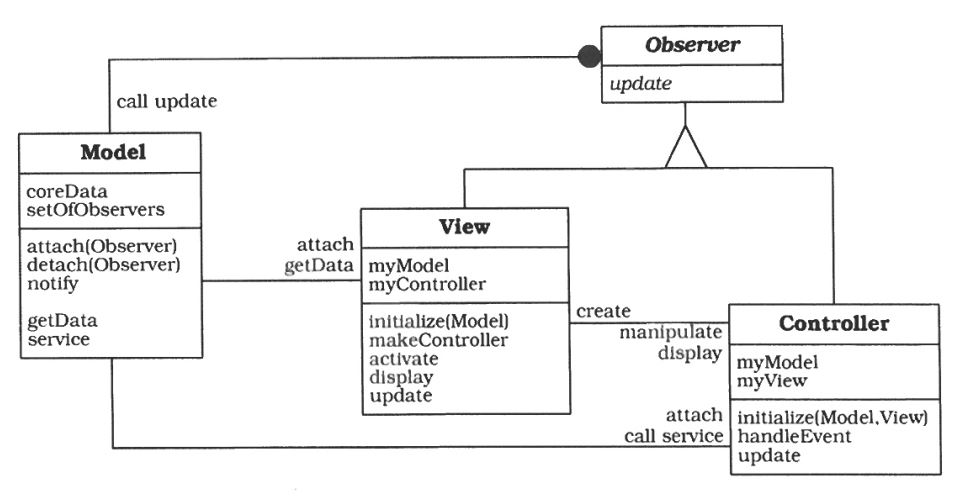
\includegraphics[width=\textwidth]{imagenes/MVC}
	\caption{Estructura b\'asica del patr\'on Model-View-Controller.}
	\label{fig:mvcdiagrama}
\end{figure}
El modelo contiene el n\'ucleo funcional de la aplicaci\'on, encapsula los datos y exporta procedimientos que realizan el procesamiento espec\'ifico de la aplicaci\'on. Los controladores llaman a esos procedimiento en nombre del usuario. El modelo tambi\'en provee funciones para el acceso a los datos que contiene, las cuales pueden ser utilizadas por los componentes de las vistas para adquirir los datos a mostrar \cite{patarq}. El mecanismo de propagaci\'on de cambios mantiene registro de todos los componentes que dependen del modelo dado que las vistas y los controladores necesitan ser informados de los cambios ocurridos en \'el. Los cambios realizados en el estado del modelo disparan el mecanismo de propagaci\'on de cambios, siendo este mecanismo el \'unico \textit{link} entre el modelo y los controladores de vistas. Las responsabilidades del modelo son: implementar el n\'ucleo funcional de la aplicaci\'on, registrar las vistas y controladores dependientes de \'el y notificar los cambios sobre los datos que maneja.

Las vistas presentan la informaci\'on al usuario, diferentes vistas pueden mostrar los mismos datos de formas alternativas. Cada vista define un procedimiento de actualizaci\'on el cual es activado por el mecanismo de propagaci\'on de cambios. Cuando el procedimiento de actualizaci\'on es llamado, la vista obtiene los datos del modelo y los muestra por pantalla. Durante la inicializaci\'on todas las vistas son asociadas con el modelo y registradas en el mecanismo de propagaci\'on de cambios. Cada vista utiliza sus propios controladores para lograr la interacci\'on con el modelo y manipular la visualizaci\'on de los datos \cite{patarq}. Las responsabilidades de las vistas son: crear e inicializar el controlador asociado a ella, mostrar la informaci\'on al usuario, implementar un procedimiento de actualizaci\'on, obtener los datos del modelo, permitir la actualizaci\'on (de ser necesario) de los datos mostrados.

Los controladores manejan los \textit{inputs} del usuario como si fueran eventos. Se puede decir que cada controlador implemente un procedimiento de \textit{event-handling} el cual es llamado en cada evento relevante a la vista. Estos eventos son transformados en requerimientos al modelo o a la vista asociada al controlador \cite{patarq}.
En el caso de que el comportamiento del controlador dependa del estado del modelo, este debe estar asociado con el mecanismo de propagaci\'on de cambios. Las responsabilidades de los controladores son: aceptar los \textit{inputs} del usuario como eventos, transformar esos eventos en requerimientos a servicios del modelo o la vista, implementar un procedimiento de actualizaci\'on de ser necesario.

\begin{figure}
	\centering
	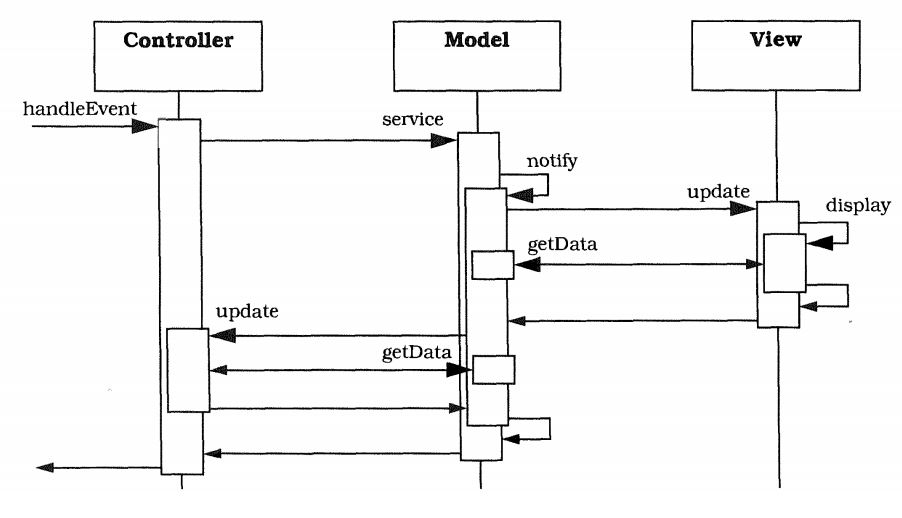
\includegraphics[width=300px]{imagenes/MVC2}
	\caption{Diagrama de secuencia: comportamiento general MVC.}
	\label{fig:mvc2}
\end{figure}

En la figura \ref{fig:mvc2} se detalla en un escenario en particular el comportamiento general del patr\'on.
Primero el controlador recibe el \textit{input} del usuario, procesa el evento y llama a un procedimiento del modelo el cual ejecuta el servicio requerido generando cambios en los datos que maneja. Luego el modelo notifica a todas las vistas y controladores, y registra los cambios por medio del mecanismo de propagaci\'on de cambios, llamando a los respectivos procedimientos de actualizaci\'on. Seguido a esto las vistas solicitan al modelo los datos actualizados y refresca la informaci\'on que muestra. Opcionalmente el modelo puede enviar datos al controlador para actualizar sus funcionalidades. La traza de ejecuci\'on finaliza retornando al controlador original.
\newpage
\section{Teor\'ia de Cromatograf\'ia}

\subsection{Teor\'ia Principal}
La ciencia que se encarga de estudiar los diferentes componentes de una sustancia es la qu\'imica anal\'itica. La t\'ecnica que m\'as se utiliza para separar los componentes en una mezcla para que esta se analice, se llama cromatograf\'ia. La mezcla b\'asicamente se trata sobre un soporte (papel o tela por ejemplo), dejando que la misma corra y seg\'un las diferentes velocidades de cada componente, los mismos se separan. El hecho de que los componentes se muevan a diferentes velocidades se debe a las diferentes fuerzas de adsorci\'on. Y se dice adsorci\'on cuando una sustancia se introduce dentro de la estructura de otra sustancia, un ejemplo claro de dicha definci\'on se da al lograr que una esponja absorba agua y si cortamos la esponja en pedazos, se encontrar\'a agua. En diferentes perspectivas, en la absorci\'on no introduce  la sustancia al volumen sino que solo se adhiere a la superficie, por ende la adsorci\'on es un fen\'omeno superficial. 
Teniendo en cuenta los nuevos t\'erminos introducidos se puede decir que la cromatograf\'ia es una separaci\'on f\'isica de los componentes de una mezcla basado en la adsorci\'on selectiva de los componentes de la mezcla al moverse por un soporte. El fin de la cromatograf\'ia es separar los componentes de una mezcla para medir la proporci\'on de cada elemento. 
La t\'ecnica de la cromatograf\'ia se aplica en dos fases:
\begin{itemize}
	\item Fase est\'atica, la mezcla se coloca sobre un soporte fijo.
	\item Fase m\'ovil, se mueve otra sustancia sobre la mezcla ya presente en la fase est\'atica, en el soporte. Es durante esta fase donde se inicia el proceso de separaci\'on de componentes.
\end{itemize}

\subsection{Diferentes Usos del An\'alisis Cromatogr\'afico}
La cromatograf\'ia tiene diferentes usos en todas sus clasificaciones:
\begin{itemize}
	\item Metilaci\'on de \'acidos grasos en el an\'alisis de aceite.
	\item An\'alisis industriales.
	\item An\'alisis forenses bromatol\'ogicos.
	\item An\'alisis toxicol\'ogicos.
	\item An\'alisis cl\'inicos.
	\item An\'alisis de contaminaci\'on ambiental.
	\item Separaci\'on de iones interferentes en an\'alisis cl\'asicos.
	\item Separaci\'on de iones de caracter\'isticas  similares.
	\item Desmineralizaci\'on del agua.
	\item Preparaci\'on de disoluciones.
	\item Disoluci\'on de sustancias insolubles.
	\item Fraccionamiento de prote\'inas.
	\item Determinaci\'on de grado de pureza.
	\item Seguimiento de reacci\'on.
	\item Determinaci\'on de amino\'acidos o prote\'inas en una soluci\'on.
	\item Aplicaci\'on sobre alimentos y productos naturales.
\end{itemize}

\section{Aplicaci\'on Espec\'ifica: TLC}
La cromatograf\'ia en capa fina (TLC) es un m\'etodo de cromatograf\'ia en el plano. Se emplea una capa plana y delgada que a la vez es el soporte o que recubre una superficie (vidrio, pl\'astico). La fase m\'ovil se mueve a trav\'es de la fase estacionaria por capilaridad, es una t\'ecnica r\'apida, de buena resoluci\'on y m\'as sensible que la cromatograf\'ia en papel. 
Se han reportados grandes avances en la producci\'on de biodiesel por medio de reacciones de transesterificaci\'on \footnote{La transesterificaci\'on es el proceso de intercambiar el grupo alcoxi de un alcohol. Es un proceso utilizado en la producci\'on de biodi\'esel.} y operaciones de tratamiento de aceites destinadas al consumo humano. La t\'ecnica de TLC resulta de gran importancia para seguir las reacciones correspondientes y medir el nivel de producci\'on.
El objetivo principal de la implementaci\'on de la t\'ecnica de TLC es la determinaci\'on de la composici\'on de los compuestos lip\'idicos que conforman la mezcla oleosa interviniente en la transesterificaci\'on para la producci\'on de biodiesel.
Las ventajas de seguir este procedimiento son la rapidez y el bajo costo de los ensayos experimentales en capa fina. La cromatograf\'ia en capa fina es una herramienta muy \'util para controles de calidad y pureza de productos. A su vez, encuentra una extensa aplicaci\'on en laboratorios industriales.
En lo que respecta al resultado final de aplicar la t\'ecnica de TLC, comparando el \'area de la mancha del est\'andar con la del analito, se puede hacer una estimaci\'on cuantitativa de la cantidad del componente presente. Los mejores resultados se obtienen cuando se raspa la mancha de la placa, se extrae el analito del s\'olido que forma la fase estacionaria, y se determina el analito por alg\'un m\'etodo f\'isico o qu\'imico adecuado. Un tercer procedimiento consiste en utilizar un densit\'ometro de barrido que puede medir la radiaci\'on emitida de la mancha por fluorescencia o reflexi\'on. Actualmente, el an\'alisis digital de la capa fina es la t\'ecnica m\'as precisa y aplicada.
Para el an\'alisis cuantitativo de la corrida cromatográfica de TLC, se debe procesar la placa digitalmente por alg\'un medio \'optico-digital, como ser un scanner, y luego procesar la informaci\'on con un software apropiado. El software \textit{Scion Image} de la Empresa \textit{Scion Corporation (ScionCorp, 2010)} ha mostrado un alto grado de desenvolvimiento para el procesamiento de im\'agenes obtenidas por TLC lo que permite obtener informaci\'on sobre la intensidad de color de la imagen, y esto puede ser relacionando con la concentraci\'on de los compuestos lip\'idicos. Para el procesamiento de los datos obtenidos, el software \textit{Matlab 7.8} de la empresa \textit{MathWorks} presenta un gran n\'umero de herramientas anal\'iticas, lo que permite obtener la variaci\'on de la concentraci\'on de los compuestos lip\'idicos respecto al corrimiento mostrado en la placa TLC.

\section{Herramientas}
\subsection{Entornos de Desarrollo Integrado}
Un Entorno de Desarrollo Integrado (IDE) es una aplicaci\'on (\textit{Software}) que brinda muchas facilidades a los programadores en el desarrollo de sistemas. Un IDE consiste normalmente de un editor de c\'odigo, un compilador y/o int\'erprete, un depurador y hasta un constructor de interfaz gr\'afica. La mayor\'ia de los IDEs modernos poseen herramientas de auto-completado inteligente de c\'odigo, brindan soporte a diversos lenguajes de programaci\'on, poseen navegador de clases y paquetes, refactorizaci\'on  inteligente de c\'odigo entre otros.

Los IDEs m\'as complejos brindan la posibilidad de anexarle \textit{Software} de terceros en forma de \textit{plug-ins} brindando extensibilidad funcional como control de versiones, generadores de casos de pruebas, pruebas unitarias, analizadores de memoria, an\'alisis de c\'odigo en tiempo de ejecuci\'on, constructores de interfaz avanzados, etc.

\subsubsection{NetBeans Java IDE}
\textit{NetBeans} es un entorno de desarrollo integrado libre, hecho principalmente para programar en Java, aunque tambi\'en soporta diversos lenguajes como \textit{PHP},\textit{ C/C++} y \textit{HTML5} junto a \textit{JavaScript} y \textit{CSS}. \textit{NetBeans} est\'a escrito en Java y puede ser ejecutado en \textit{Windows, OS X, Linux, Solaris} y cualquier otra plataforma que sea compatible con la \textit{JVM (Java Virtual Machine)} \cite{netbeans}. Fue desarrollado inicialmente en el a\~no 2000 por \textit{Sun MicroSystem} como un proyecto de \textit{Software} libre el cual contin\'ua en desarrollo y crecimiento por una comunidad de desarrolladores junto a \textit{Oracle Corporation}.
\textit{NetBeans} est\'a dise\~nado en forma modular, por lo que cada funci\'on del sistema esta provista por un modulo en particular. De esta forma el usuario puede agregar sus propios m\'odulos al sistema (respetando una API descrita por el IDE) o bien puede obtenerla del repositorio de \textit{plug-ins online}.